\section{Task 5: Evaluation}

\subsection*{Task 5A: Characteristics of Evaluation Metrics}

Mean Squared Error (MSE) and Mean Absolute Error (MAE) are two standard metrics for evaluating regression models. Their formulae are:

\[
\text{MSE} = \frac{1}{n} \sum_{i=1}^{n} (y_i - \hat{y}_i)^2
\qquad\qquad
\text{MAE} = \frac{1}{n} \sum_{i=1}^{n} |y_i - \hat{y}_i|
\]

where $y_i$ is the actual value, $\hat{y}_i$ is the predicted value, and $n$ is the number of samples.

The key difference between them comes down to how they treat large errors. MSE squares each error before averaging, which means a single prediction that is off by 40 points gets penalized 16 times more than one that is off by 10. MAE treats both proportionally, so the same pair of errors contributes only 4 times more. In practice, this means MSE is more sensitive to outliers. If the goal is to minimize worst-case errors or if large mistakes are especially costly, MSE is the better choice. If all errors matter equally regardless of size, MAE gives a more representative picture of typical model performance.

There is also an optimization angle. MSE is differentiable everywhere, which makes it easier to use with gradient-based training methods. MAE has a non-differentiable point at zero, which can cause issues during optimization. This is one reason why MSE is more commonly used as a training objective even when MAE might be the preferred evaluation metric.

MSE and MAE produce identical results when every prediction error has exactly the same magnitude. Consider a simple example: a model predicts housing prices for 4 houses, and every prediction is off by exactly 10{,}000 euros. In that case, $\text{MAE} = 10{,}000$ and $\text{MSE} = 100{,}000{,}000$. The values differ, but both metrics agree perfectly on which model is better because neither is affected by variance in the error distribution. There is no variance. If a second model also makes uniform errors but of size 12{,}000, both MSE and MAE will rank the first model higher.

More formally, MSE can be decomposed as $\text{MSE} = \text{MAE}^2 + \text{Var}(\text{errors})$ when errors are all the same sign. When the variance of the error distribution is zero (all errors equal), the two metrics carry the same information and will always rank models identically. They start to disagree when one model has high error variance, meaning a mix of small and large mistakes, because MSE penalizes the large ones disproportionately while MAE does not.

\subsection*{Task 5B: Impact of Evaluation Metrics}

Table~\ref{tab:task5_metrics} shows the MSE and MAE values for both regression models from Task 4.

\begin{table}[h]
\caption{MSE and MAE comparison for Ridge and Random Forest on stress prediction.}
\label{tab:task5_metrics}
\centering
\begin{tabular}{|l|r|r|r|r|r|}
\hline
Model & MSE & RMSE & MAE & Median AE & Max AE \\
\hline
Ridge & 691.32 & 26.29 & 22.52 & 20.45 & 45.82 \\
Random Forest & 825.01 & 28.72 & 25.18 & 23.45 & 56.97 \\
\hline
\end{tabular}
\end{table}

Ridge outperforms Random Forest under both metrics, but the gap is not the same. The MSE difference between the two models is 133.69 (a 19.3\% increase from Ridge to Random Forest), while the MAE difference is only 2.66 (an 11.8\% increase). MSE amplifies the gap because Random Forest makes a few large errors that get squared. Its worst prediction is off by nearly 57 points, compared to Ridge's worst at about 46 points. That single outlier error contributes disproportionately to MSE.

Figure~\ref{fig:task5_breakdown} shows the per-sample absolute errors sorted from largest to smallest for both models. The darker bars represent absolute errors (what MAE averages), while the lighter overlay shows the squared errors scaled to the same axis. For both models, the top 5 largest errors account for roughly 40 to 43\% of the total MSE but only about 29\% of the total MAE. This demonstrates exactly how MSE amplifies the influence of outlier predictions.

\begin{figure}[h]
\centering
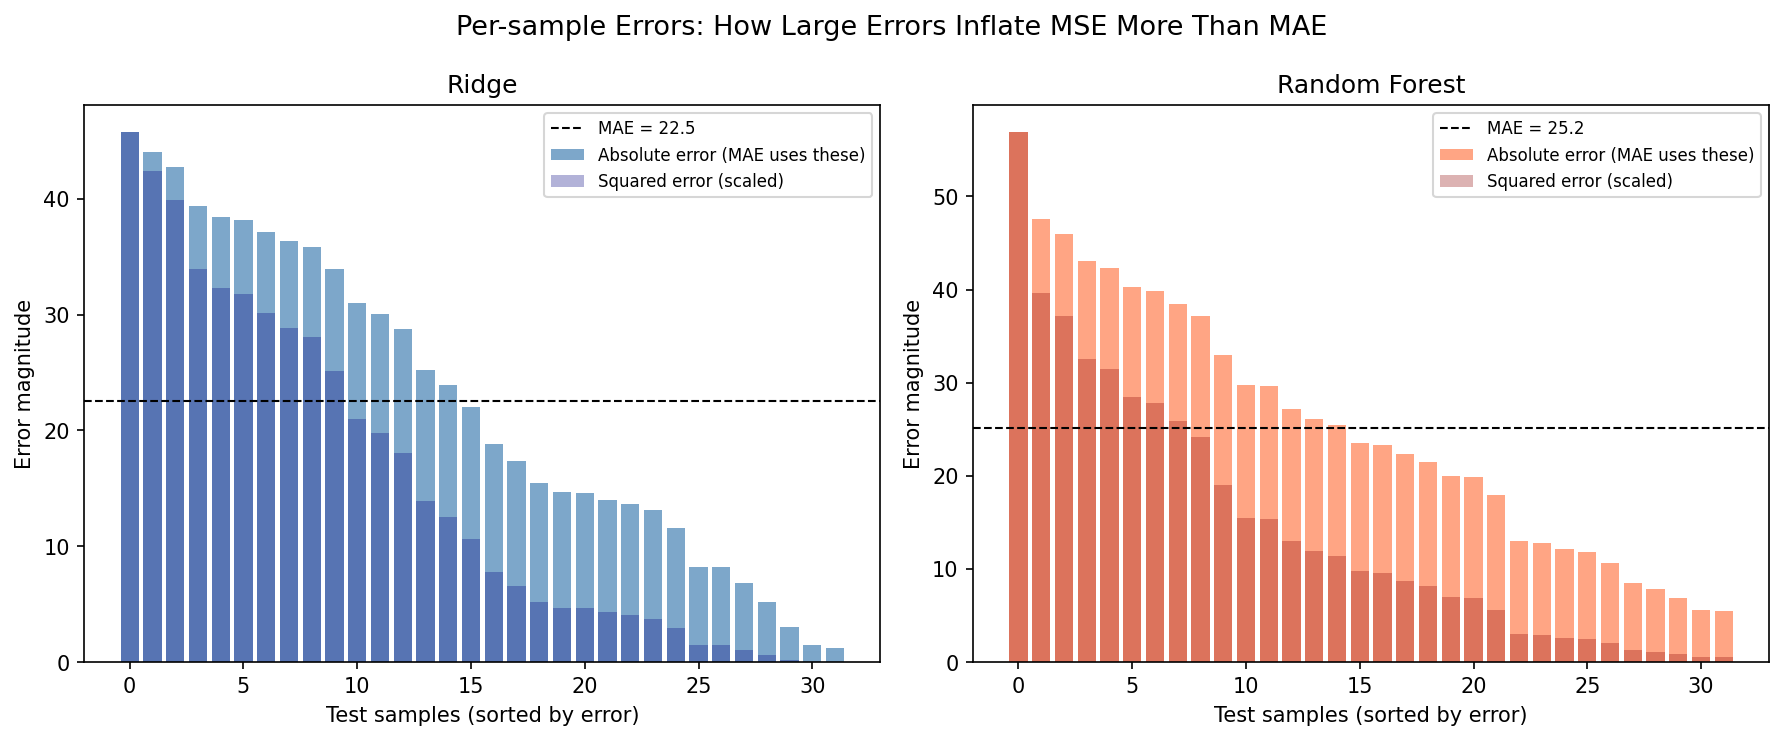
\includegraphics[width=\textwidth]{task5/task5_error_breakdown.png}
\caption{Per-sample errors sorted by magnitude, showing how large errors contribute disproportionately to MSE compared to MAE.}
\label{fig:task5_breakdown}
\end{figure}

For this particular problem, MAE is arguably the more useful metric. Stress is self-reported on a subjective scale, so the data itself contains noise. A prediction that is off by 40 points is not necessarily four times worse than one that is off by 20, it could just reflect inconsistent self-reporting. MAE treats these errors more evenly and gives a more intuitive summary: on average, the model's predictions are about 22 to 25 points away from the actual stress value. That is easy to interpret on a 0 to 100 scale.

That said, MSE still adds value as a complementary metric. The fact that Ridge has a noticeably lower MSE tells us it avoids the extreme mispredictions that Random Forest occasionally makes. If the application required reliable worst-case behavior, MSE would flag Random Forest's weakness more clearly than MAE does.
